% Koma-Script Basisklasse
\documentclass[a4paper,12pt,pagesize,headsepline,bibtotoc,titlepage]{scrartcl}

\usepackage[english]{babel}		% deutsche Trennmuster
\usepackage[utf8]{inputenc}		% direkte Eingabe von Umlauten & Co. (Vorsicht: Encoding im Editor muss auch UTF-8 sein!)

\usepackage[T1]{fontenc}			% T1-Schriften

\usepackage{mathptmx}			% Times/Mathe \rmdefault
\usepackage[scaled=.90]{helvet}	% Skalierte Helvetica \sfdefault
\usepackage{courier}			% Courier \ttdefault

% Zusatzpakete für mehr mathematische Symbole, Einfügen von Grafiken 
% und bessere Bildunterschriften
\usepackage{amsmath,amsthm,amsfonts,graphicx,caption,subcaption}

% Wenn man direkt mit dem pdflatex eine PDF-Datei erzeugt, sollten diese beiden Pakete eingebunden werden
\usepackage{hyperref} % Hyperlinks anklickbar
\usepackage{ae,aecompl} % bessere Bildschirmschriftarten usw.
\usepackage{epstopdf} % support eps 

\pagestyle{headings}

% Abstand der Kopfzeile vom Text:
\headsep4mm

\typearea[current]{current}     % Satzspiegel neu berechnen

% andere Bildunterschrift mit Hilfe von caption
\renewcommand{\figurename}{Abb.}
\renewcommand{\captionlabelfont}{\bf}

\title{
	\includegraphics*[width=0.4\textwidth]{hpi_logo_2017.eps}\\
	\vspace{24pt}
	Text Localization with Deep Reinforcement Learning
}
\subtitle{
	Lecture\\
	Machine Intelligence with Deep Learning\\
	Winter term 2018/2019
}
\author{
	Bastian König, Federico Malerba, Kolya Opahle\\
	Jona Otholt, Milan Proell\\[12pt]
	Supervisors:\\
	Christian Bartz,\\	
	Dr. Haojin Yang
}
\date{February 28, 2019}

\begin{document}
\maketitle
\tableofcontents
\newpage


\section{Section heading}
Lorem ipsum dolor sit amet, consectetur adipiscing elit. Morbi sed nunc leo. Nam ac leo venenatis est commodo vehicula. Nulla justo nisl, venenatis id tincidunt id, porta ut felis. Cras eu justo ac nisi ornare commodo placerat at risus. Suspendisse ut urna tellus. Cras ut erat tempus justo aliquam laoreet. Praesent est neque, interdum quis convallis et, gravida sed arcu. Mauris bibendum, dui at ullamcorper luctus, arcu dolor laoreet nisi, ut facilisis dui enim a nisl. Sed odio risus, pulvinar suscipit feugiat pharetra, varius non est. Morbi pellentesque libero eu odio pulvinar semper. Praesent cursus adipiscing metus nec fermentum. Nullam malesuada euismod mi nec tincidunt. Nulla eget auctor velit. Mauris quam odio, blandit sit amet pharetra non, lobortis sed risus. Aliquam nec orci vel dolor suscipit tristique. Etiam quam eros, commodo at iaculis at, molestie eu metus. Maecenas viverra dui non magna suscipit sodales commodo justo iaculis (siehe Abbildung \ref{fig:test}).

\begin{figure}[hbp]
\begin{center}
\includegraphics*[width=0.75\textwidth]{example.png}\\
\caption{A figure, Source: \cite{caicedo2015active}}
\label{fig:test}
\end{center}
\end{figure}

\subsection{Section heading}
Quisque pharetra, tellus id cursus consectetur, libero arcu sollicitudin nisl, in pulvinar tortor tortor consequat arcu. Donec pulvinar nibh in elit iaculis vel pellentesque diam tincidunt. Fusce posuere volutpat libero in consequat. Curabitur sit amet interdum leo. Vestibulum massa ante, ultrices vel dictum vitae, vestibulum consequat magna. Pellentesque turpis ligula, fermentum vel consectetur id, ornare non diam. Lorem ipsum dolor sit amet, consectetur adipiscing elit. Vestibulum pretium scelerisque nisi sit amet semper. Nulla lobortis quam sit amet turpis tristique accumsan. Vivamus sed nunc odio.

In tempor leo ut lectus lacinia commodo. Vestibulum pretium accumsan erat, non interdum sem feugiat a. Praesent tempor odio quis arcu laoreet dignissim. Mauris egestas lectus sed purus malesuada feugiat. Lorem ipsum dolor sit amet, consectetur adipiscing elit. Donec placerat auctor laoreet. Nunc hendrerit viverra posuere. Morbi egestas ante et augue mattis eleifend. Aliquam nibh turpis, adipiscing ac lacinia sed, laoreet vel orci. Donec velit est, fringilla ac vulputate vitae, commodo a velit. Fusce vitae posuere diam. Pellentesque tellus tellus, volutpat non fringilla in, vulputate vitae magna. Proin ligula diam, aliquet eget feugiat ac, rutrum in tortor.
\section{Related work}

Before we explain the reinforcement learning approach to text
detection, we give a short overview over the state of the art methods
in text localization in this section. First, we briefly discuss
methods that use handcrafted features to then then move on to more
recent approaches that use convolutional neural networks.

Approaches that rely on handcrafted features often make use of visual properties specific to text to distinguish it from 
the background or other objects. These are then used to generate candidates for further examination \cite{zhu2016scene}. One such property is that 
the stroke width of a character is usually almost constant. The so called Stroke Width Transform (SWT) operator makes use of this finding to assign 
to each pixel the width of the stroke associated with it \cite{epshtein2010detecting}. By grouping pixels based on these values, letter candidates 
are generated, which are then filtered and aggregated to text lines.

Another way of generating candidates is the Maximally Stable Extremal Regions (MSER) approach \cite{neumann2010method}. This method exploits that 
all pixels belonging to a letter usually have a similar colour and intensity. Similar to the previous method, candidates are generated by identifying
regions of similar intensity. A classifier is then used to filter out candidates that do not contain a letter and the remaining candidates are
aggregated into lines.

The emergence of convolutional neural networks provides an alternative to handcrafting features, as it is now feasible to learn directly from the 
image itself. This has been used for text detection in various ways that are often inspired by developments in the more general field of object 
detection. An example of this is the Rotating Region Proposal Network \cite{ma2018arbitrary} that builds on the Faster R-CNN object detection 
mechanism \cite{ren2015faster}. Faster R-CNN first feeds the image into a convolutional neural network that outputs a feature map, meaning that the 
features are not constructed by human reasoning but learned during training. This feature map is then used as the input for another network that 
generates region proposals. These proposals serve a role similar to that of the candidates in the previous methods. In the last step, 
the proposals are assigned both a class and an offset that slightly adjusts the bounding box to better fit the object. The Rotating Region Proposal
Network adapts this method to text localization by enabling the network to propose bounding boxes with varying orientations as opposed to 
axis-aligned bounding boxes.

Faster R-CNN yields good detection results, but the two-step process of first creating and then validating region proposals is time consuming. The 
Single Shot MultiBox Detector (SSD) approach \cite{liu2016ssd} addresses this issue by skipping the region proposal creation phase and instead
performing the entire detection process in one network. This results in higher execution speed while achieving better detection results. Just like 
Faster R-CNN, SSD has been adapted for text localization. One approach that is inspired by SSD is Textboxes++ \cite{liao2018textboxes++}. Compared to 
SSD, Textboxes++ improves recognition of objects with extreme aspect ratios, which are common in text localization. Unlike SSD, it is also able 
to recognize arbitrarily oriented text.
\section{Theoretical Background}\label{sec:theoretical background}

As previously stated, our approach relies on reinforcement learning to achieve its goal of text localization. It is therefore important before we continue to quickly go through the basic ideas and notations behind this area of machine learning\footnote{What follows is meant to be only a brief introduction to the concepts pertinent to our application,  further details about the model and the mathematical concepts behind it can be found in a number of resources among which we suggest the book by Sutton and Barto \cite{Sutton:1998:IRL:551283}.}.

In every reinforcement learning application there are two basic building blocks that essentially define the entire system: the environment and the agent. The setup allows us to find intelligent solutions to problems which have no clear optimal strategy; we do this by exploring the environment and discovering which actions are best to take. Much of what is going to be described is not at all rigid, and various implementations of reinforcement learning models are applied modifying either the structure of the environment, of the agent or of the input to the agent.

The environment describes the space the agent operates in; it defines where the agent can be, what it can do and what is good or bad for the agent. More precisely, the environment is defined by a set of states $S$ in which the agent can be, by a set of actions $A$ which the agent can take in these states and by a reward function $R$. It is important to note that the set of actions can be constant across all state or it can be different depending on which state the agent is in, furthermore the agents transitions between states - though dependent on the action taken and the current state - can have a stochastic nature to them. The reward is a function which depends on the current state, the action taken and the final state; it is calculated step by step and fed back to the agent so that it may learn what is best to do in the given environment.

The agent is a general machine learning model (in our case a Deep Neural Network) which takes as input a representation of the current state. In general, the agent aims at maximizing the reward it gains from the environment; this means that it has to determine a policy $\pi$ which determines the action to be taken at a certain state in order to maximize the expected future reward. This policy need not be deterministic and in fact it is defined as 
$$\pi: S \times A \to [0,1]$$
$$\pi(a|s) = P(a_t = a|s_t =s)$$
To determine this policy the agent needs to explore the $S \times A$ space and keep track of the rewards received to understand what is best to do in each state. It is important to note that the agent doesn't merely try to maximize the reward for the contingent action, but its aim is to obtain the highest possible total reward. This means that the effect of the current action on future rewards is also considered in order to establish the optimal policy.


\newpage


\subsection{Previous implementation}
Our application was in large part inspired by the work done by Caicedo and Lazebnik in their paper published in 2015 \cite{caicedo2015active}; in this paper an interesting way of applying reinforcement learning to object detection is laid out.

The state representation fed to the agent as input is a tuple composed by a feature vector $o$ and a history vector $h$ of previous actions taken. The vector $o$ is obtained by applying a feature extractor (CNN) to the current portion of the image that the agent is looking at; this is done after having properly warped it to match the 224x224 input of the CNN. The vector $h$ keeps track of the past 9 actions and is meant to inform the agent on what has happened in the past.

The agent is set to be a Deep Q-Network \cite{mnih2015human} with 2 hidden layers which outputs the selected action for the given input. It begins by looking at the entire image and can take 9 different actions (Figure \ref{fig:environment-actions-from-base-paper}) to change what it looks at. One of these 9 actions is the \textit{trigger} action, and the portion of the image the agent is looking at when pulling the \textit{trigger} is considered as the proposed bounding box for the object. The 8 remaining actions modify the image and use a parameter $\alpha = 0.2$ so that transformations have magnitude relative to the size of the currently considered bounding box; this is done to maintain the action space simple and adaptable to the needs of the agent.

\begin{figure}[h!]
    \centering
    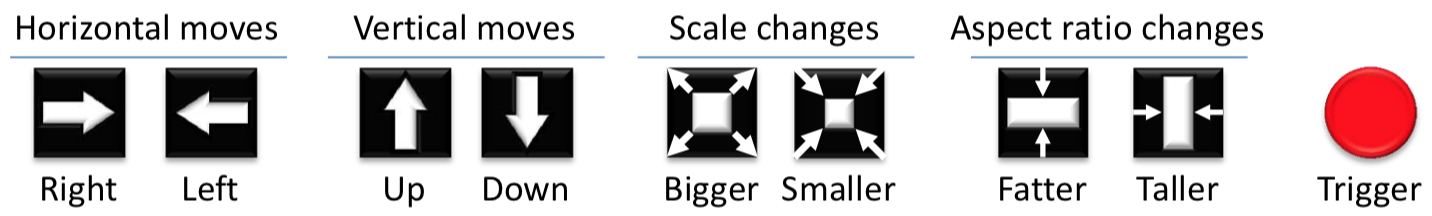
\includegraphics[width=0.7\textwidth]{figures/environment-actions-from-base-paper.png}
    \caption{The actions offered by the environment to the agent\cite{caicedo2015active}}
    \label{fig:environment-actions-from-base-paper}
\end{figure}

The reward function at each step considers the variation of the intersection over the union metric (IoU) and rewards the agent with a discrete $\pm 1$ depending on whether it has improved or not. For the \textit{trigger} action the reward is $\pm 3$ depending on whether the IoU is above a certain threshold. The reasoning behind these rewards is best explained in the paper to which we refer for further explanations and details.

Limits on the duration of episodes and resetting behaviours for the environment are also implemented in the paper in order to avoid situations in which the agent might get lost and lose time for no reason.


\section{System architecture}

The system consists mainly of three parts, of which one is used for generating test data and two are used for the actual reinforcement learning.
On the one hand, there exits a Python-based program that can be used to generate synthetic training images with text on them.\footnote{The program's source code can be found on GitHub.\cite{GitHubDatasetGenerator}}. 
This program is called the \textit{dataset-generator}.
On the other hand, there exist two programs also based on Python which provide both the environment and the agent used for the reinforcement learning's training and testing.\footnote{The source code of those programs can be found on GitHub as well.\cite{GitHubTextLocalizationEnvironment}\cite{GitHubTextLocalizationAgent}}. 
Those programs are called \textit{text-localization-environment} and \textit{text-localization-agent} respectively. 

Both the \textit{dataset-generator} and the \textit{text-localization-agent} program use the Python package \textit{click}\cite{PythonPackageClick} for offering command-line interfaces that allow users to change the programs' parameters without having to change their source code.
This is especially useful when running the programs on computers accessed via a remote connection (e.\,g. via SSH), as it often is the case when working on machine learning projects.

A typical use-case for using the system is to (a) generate synthetic training data using the \textit{dataset-generator}, (b) installing the \textit{text-localization-environment} for later usage by the agent and (c) training and/or evaluating one or multiple agents using the \textit{text-localization-agent}. 
In the following paragraphs, the three programs and their usage options are described more in-depth.

\subsection{The dataset-generator program}\label{sec:dataset-generator}

As briefly introduced before, the \textit{dataset-generator} is a program that can be used for generating synthetic training data for usage in machine learning projects related to the bounding box detection (localization) of text on images. 
It does so by using the Python package Pillow\cite{PythonPackagePillow} to load one or multiple fonts, create images of a specific size and render one or multiple words of text onto those images.
The words themselves come from a public domain word list originally contained in the original BSD project project.\cite{BSDWordlist}

For the generation of image datasets, users can control the images' width, their height, the amount of images to generate, the location of a word list (in a format similar to the word list contained by default, as described above), a seed used for the random calculations within the program as well as whether the program should use a debug mode (in which it renders AABB outlines around the corresponding words).

Figure \ref{fig:dataset-generator-sample-output} shows two sample images created by the \textit{dataset-generator}, one using the default settings and one explicitly having the \textit{debug} flag set to true. 
In addition to the images, the program also creates a \texttt{.npy} file containing the AABB locations of the words in the images in a Numpy-encoded way as well as a \texttt{.txt} file containing the relative locations of the generated images.

\begin{figure}[h!]
    \begin{subfigure}[t]{0.5\textwidth}
        \centering
        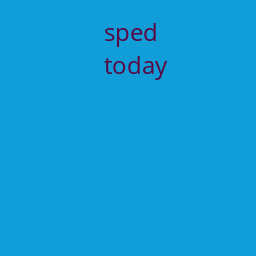
\includegraphics[width=0.8\textwidth]{figures/dataset-generator-sample-1.png}
        \subcaption{Debug mode disabled (default setting)}
    \end{subfigure}
    \begin{subfigure}[t]{0.5\textwidth}
        \centering
        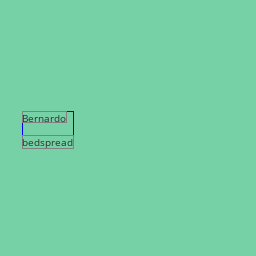
\includegraphics[width=0.8\textwidth]{figures/dataset-generator-sample-debug.png}
        \subcaption{Debug mode enabled. The blue and gray boxes indicate the AABB of the single words and of the whole “text” block}
    \end{subfigure}
    \caption{Two sample images created by the \textit{dataset-generator}}
    \label{fig:dataset-generator-sample-output}
\end{figure}

\noindent Together with the \texttt{.npy} and the \texttt{.txt} files, the images can be used by the \textit{text-localization-environment} program as described in the following section.

\subsection{The text-localization-environment program}

The \textit{text-localization-environment} program is designed to conform to OpenAI Gym's environment interface \textit{Env}\cite{OpenAIGym} by implementing the three following methods:
\begin{quote}
    \begin{itemize}
        \item reset(self): Reset the environment's state. Returns observation.
        \item step(self, action): Step the environment by one timestep. Returns observation, reward, done, info.
        \item render(self, mode='human', close=False): Render one frame of the environment. The default mode will do something human friendly, such as pop up a window. Passing the close flag signals the renderer to close any such windows.
    \end{itemize}\cite{OpenAIGymReadme}
\end{quote}
In general, the environment is based on the algorithm described in the paper\cite{caicedo2015active} which we based our research on:
The environment offers a total of 9 actions to the agent (and thus uses a \textit{discrete} action space).
Those actions are exactly the same as the one used in the paper mentioned above, and are visualized in figure \ref{fig:environment-actions-from-base-paper}.

\begin{figure}[h!]
    \centering
    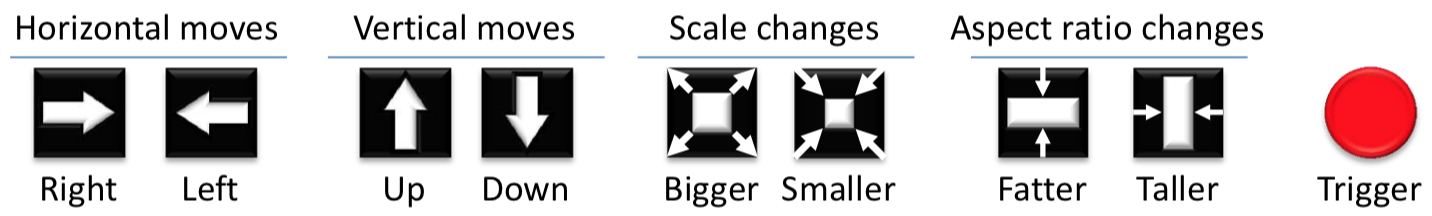
\includegraphics[width=0.7\textwidth]{figures/environment-actions-from-base-paper.png}
    \caption{The actions offered by the environment to the agent\cite{caicedo2015active}}
    \label{fig:environment-actions-from-base-paper}
\end{figure}

After being initialized with a set of images (indicated by a corresponding \texttt{.txt} file, as described above) and the ground truth bounding boxes (contained in a \texttt{.npy} file), the environment acts as a kind of state machine which can be controlled by the three main methods described above. 
For calculating the observation in the \textit{reset} and \textit{step} methods, the environment uses a feature extractor – in our case, we used VGG16\cite{VGG16} in the beginning and replaced it with ResNet\cite{ResNet} later.
In order to control whether this feature extractor runs on the GPU, the environment can be initialized with a corresponding parameter indicating the ID of the GPU to be used.

For calculating the reward returned by the \textit{step} method, the environment calculates the best intersection over union (IoU) of the current bounding box and any of the ground truth bounding boxes. 
Depending on whether this IoU changed positively or negatively in respect to the one calculated in the step before, the reward is either $+1$ or $-1$. 
During the course of the project, we also introduced two more means for increasing the likelihood of the agent using the \textit{trigger} action: We (a) made the environment count the amount of consecutive steps taken that did not change the IoU in any way (and give a negative reward of $-1$ whenever this count exceeds 3 steps) and (b) introduced a duration penalty (with a default value of $0.03$) which is multiplied by the amount of steps taken since the last time the \textit{reset} method was called and subtracted from the reward.

Although the \textit{text-localization-environment} program is theoretically independent from the agent using it (as proposed in the OpenAI specification), it usually is used together with such an agent.

The program allowing the training and testing of such agents is described in the following section.

\subsection{The text-localization-agent program}

The \textit{text-localization-agent} program uses the deep reinforcement learning framework ChainerRL\cite{ChainerRL} internally.
In addition to offering a variety of state-of-the-art deep reinforcement learning algorithms and different Q-functions, ChainerRL also offers convenience functions for training an agent while evaluating it at a given interval.

Thus, the \textit{text-localization-agent} program acts on a quite high level of abstraction:
It offers a \textit{click}-based CLI which allows users to provide an amount of steps for which a training should be run as well as the locations of the \texttt{.txt} and \texttt{.npy} files described in section \ref{sec:dataset-generator}. 
Furthermore, it allows users to specify the ID of the GPU to use (if any) and whether the intermediate training results should be logged to TensorBoard, as described in the following paragraph.

\paragraph{TensorBoard logging integration}

Although being mainly focused on being used together with TensorFlow, the TensorBoard visualization toolkit\cite{TensorBoard} also can be used for monitoring the training progress of other machine learning applications.

Since ChainerRL doesn't offer a built-in way of logging in a format suitable for visualization in TensorBoard, we had to implement a corresponding logging ourselves.
Thankfully, there exists a library called \textit{tensorboard-chainer}\cite{TensorBoardChainer} which offers a convenient way of logging variables like scalars and images to TensorBoard.
The resulting TensorBoard logging is implemented using a so-called ChainerRL step hook\cite{ChainerRLStepHooks}.
Figure \ref{fig:tensorboard-sample-output} shows a sample visualization created in TensorBoard.

\begin{figure}[h!]
    \centering
    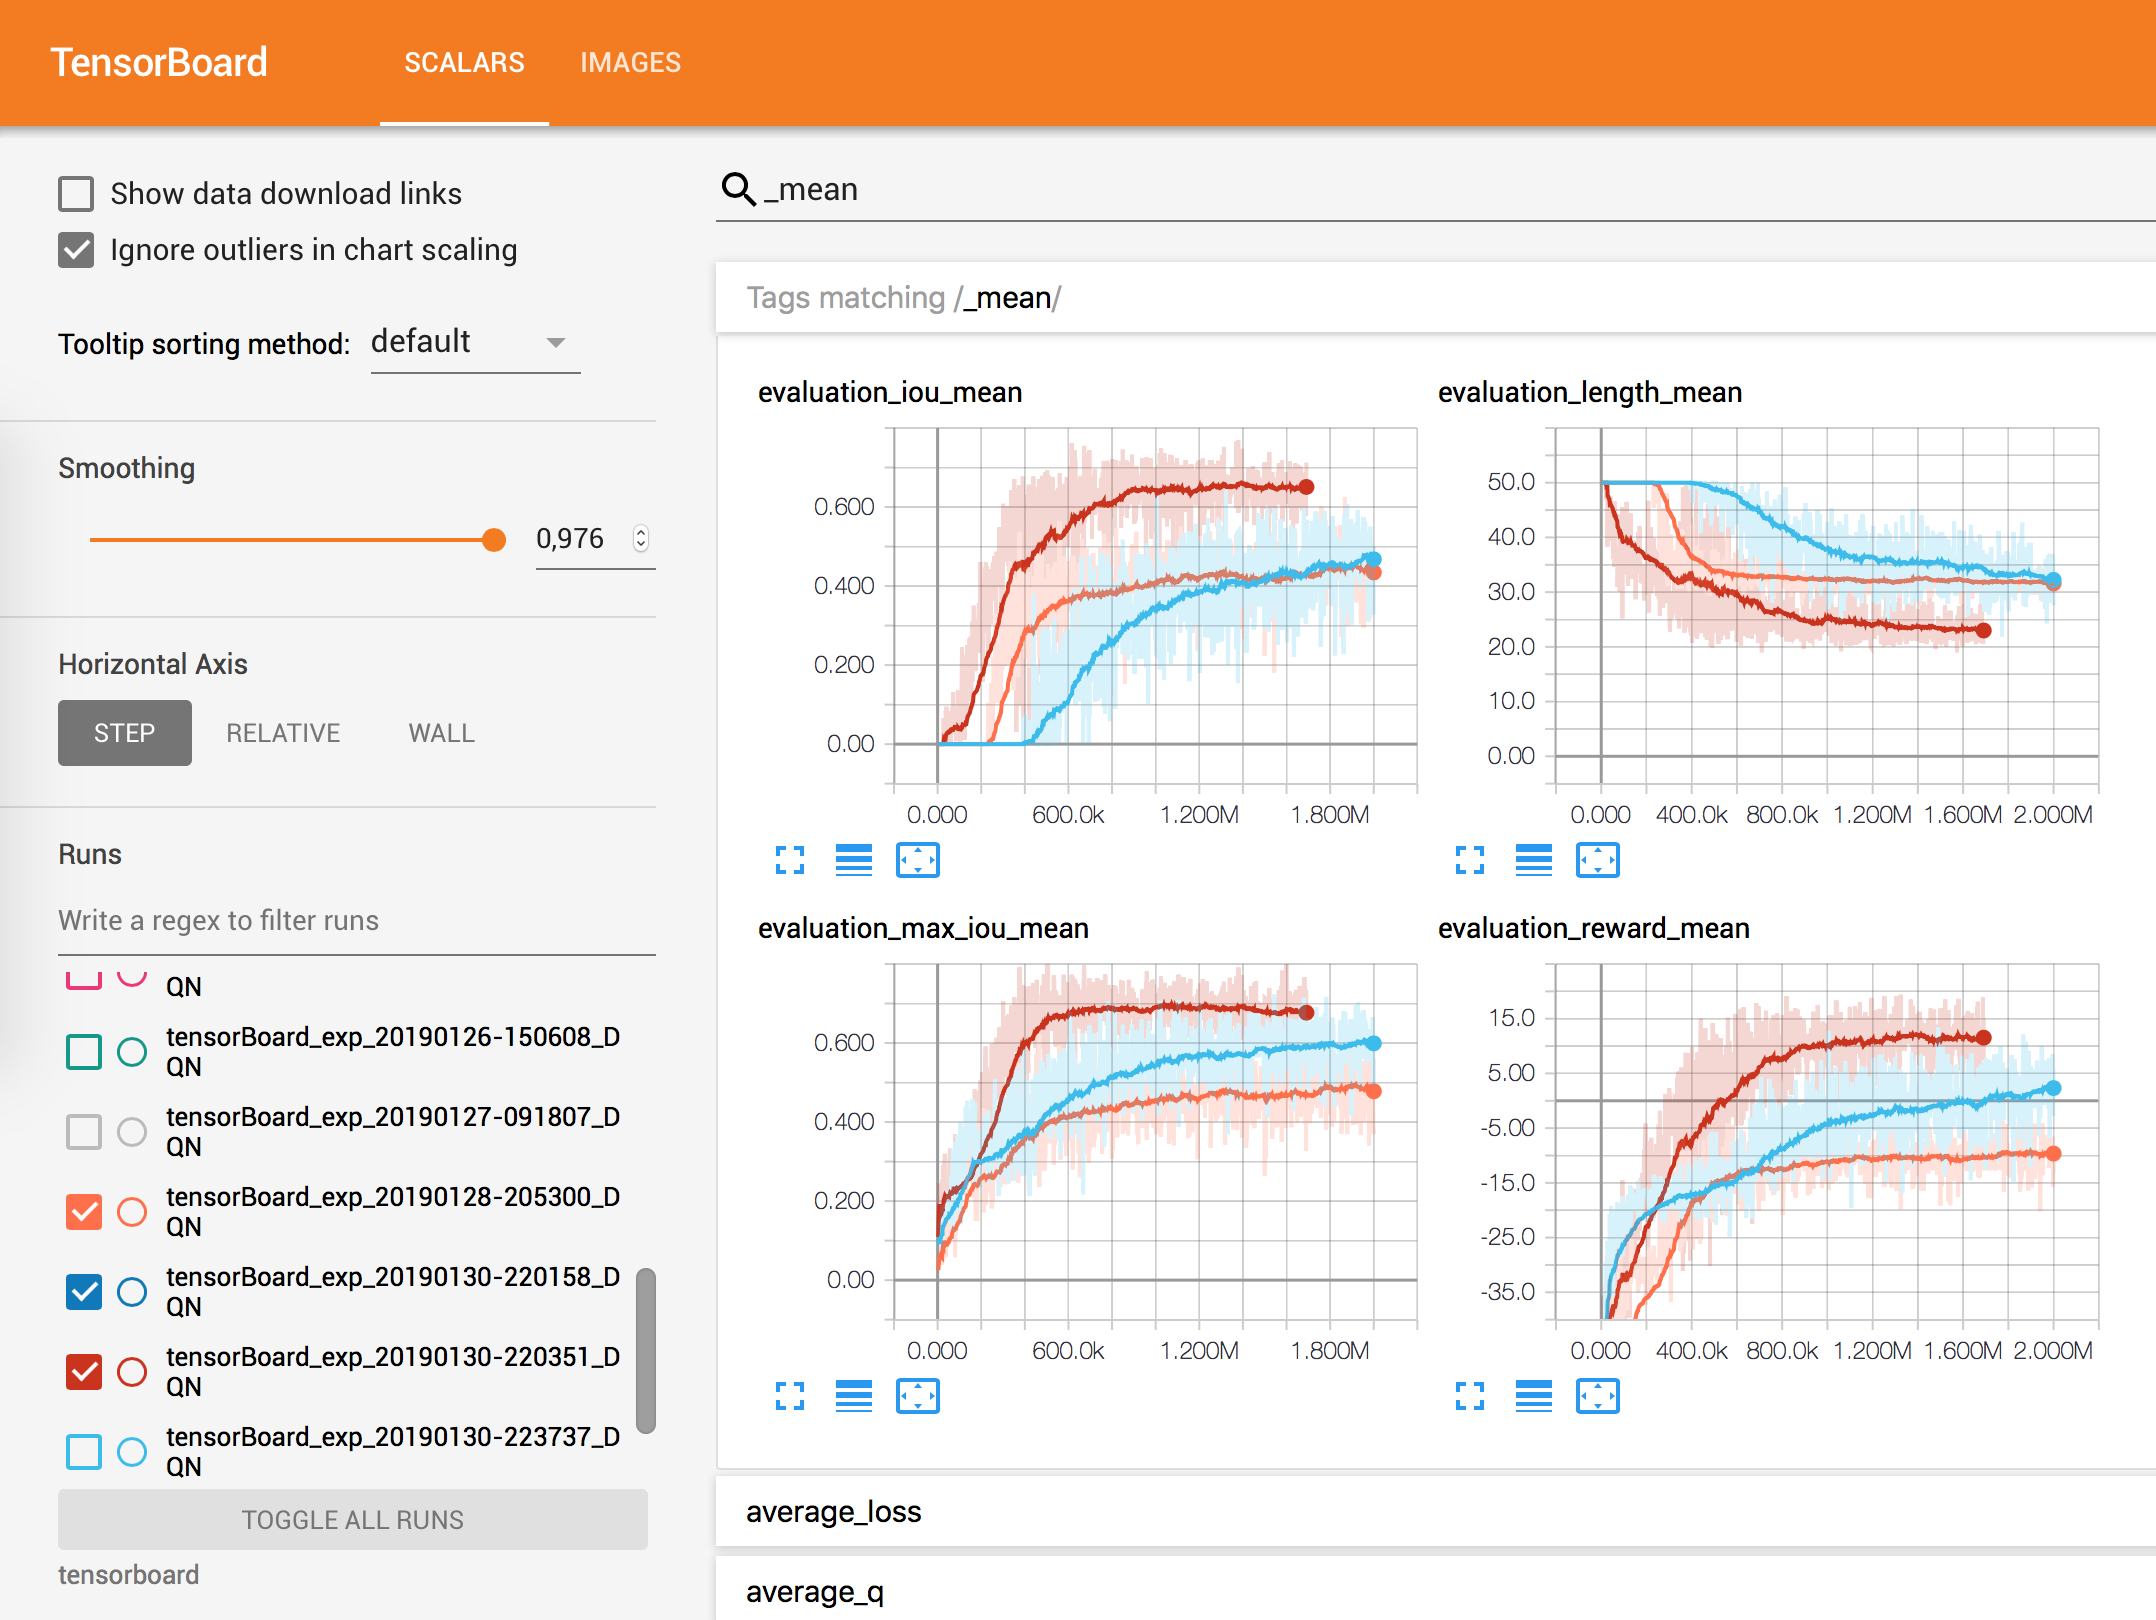
\includegraphics[width=0.55\textwidth]{figures/tensorboard-sample-output.png}
    \caption{Sample visualization created using TensorBoard}
    \label{fig:tensorboard-sample-output}
\end{figure}

\noindent We tried using the ChainerRL Visualizer\cite{ChainerRLVisualizer} as well, but it turned out to be less useful than our integration of TensorBoard.
This was mostly based on the fact that the ChainerRL Visualizer can not yet create saliency maps for models containing a RNN, as well as on the fact that the ChainerRL Visualizer requires users to control the training itself via the UI, which was in our case less practical than being able to run the training programmatically from our \textit{text-localization-agent} program.

While the visualizations in TensorBoard help to get a quick impression on how well a training run performs in comparison to others, they do not really give a formal evaluation of the agents' performances.
Thus, we implemented a Python script that allow evaluating a trained agent on a specified set of images, as described in the following paragraph.

\paragraph{Evaluation script}

In order to be able to precisely calculate the mean average precision (mAP) as well as precision and recall for specific IoU thresholds, we implemeted a small wrapper script around ChainerCV's VOC evaluation methods\cite{ChainerCVEvalDetectionVOC}.
This allows users to provide a dataset in the format created by the \textit{dataset-generator} program and calculate the mAP as well as precision and recall values based on the metrics used in the PASCAL VOC challenge.

\section{Results}\label{sec:Results}
During our experimentation with the agent we attempted using multiple different configurations for the agent and the environment.
In this section we will focus on a few significant iterations of the agent and environment that were used during the course of the project.
It will showcase the progress of our agent and inform about different decisions made to improve the agents performance.
We used the average IoU of the agent during training and the mean average precision of the agent on a test data set to evaluate agent performance during the experimentation.


\subsection{Results closest to Paper}
Our training setup for the first agent was following the paper\cite{caicedo2015active} without any modification to the suggested formula from our side.
This setup resulted in an agent which, while being able to focus on the relevant parts of the image, was not able to pull the trigger.
We think this was due to it being able to generate more reward just by hovering around the target bounding box instead of pulling the trigger, which would end the episode and consequentially stop the agent from acquiring any further reward.

\subsection{Experiment 1}
After observing the first trained agent we decided to implement a way of penalizing the agent for long episode duration.
This was done by applying a negative reward for each step taken which would in turn force the agent to end episodes earlier if he was to receive any positive reward.
Using this configuration the agent managed to focus on the correct part of the image and also managed to pull the trigger.
The resulting agent was the first to consistently finish the episodes thus achieving an average IoU of around $0.35$ in a relatively short training run, with our target IoU being $0.6$ during our testing.

\begin{figure}[h!]
    \centering
    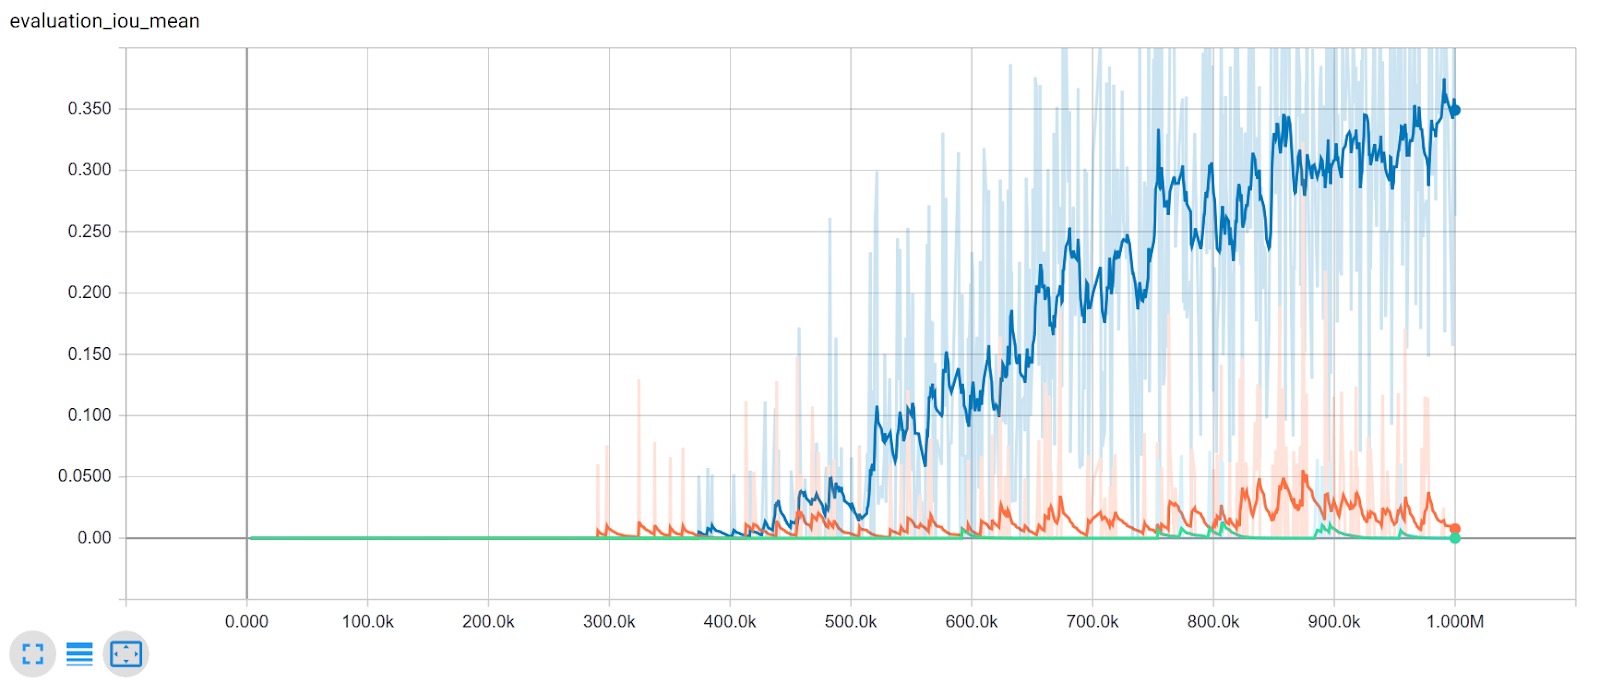
\includegraphics[width=0.7\textwidth]{figures/penalty_results.png}
    \caption{Results from the first Experiment}
\end{figure}

\subsection{Experiment 2}
During our meetings a performance discussion prompted switching the feature extractor from VGG16\cite{VGG16} to ResNet\cite{ResNet} because of ResNet's better applicability in object detection.
The feature extractor switch resulted in a pretty noticeable performance spike in comparison to the old agent.
We achieved an average IoU of $0.64$ with the same target IoU of $0.6$ as in the previous experiment and also managing a mean average precision of $92.74$ percent on our test set generated by the \textit{dataset-generator} described in \ref{sec:dataset-generator}. 

At this point it should be noted, that the average IoU is very unlikely to be substantially higher than the target IoU even with perfect precision. This is the case because under the reward scheme we used the agent has no incentive to strive for an IoU that is higher than the target, the reward will be the same. This means that to achieve an mean IoU significantly higher than the 0.64 achieved is this experiment a higher target IoU would be required.
\section{Conclusion}


\newpage
%%%% bibtex file %%%%%%
\bibliographystyle{alphadin}
\bibliography{references} 

\end{document}